\chapter{Synthesis Methods}
\label{chap:Synth}
\thispagestyle{empty}

%%%%%%%%%%%%%%%%%%%%%%%%%%%%%%%%%%%%%%%%%%%%%%%%%%%
%%%%%%%%%%%%%%%%%%%%%%%%%%%%%%%%%%%%%%%%%%%%%%%%%%%
%%%%%%%%%%%%%%%%%%%%%%%%%%%%%%%%%%%%%%%%%%%%%%%%%%%

Synthesis of perovskite oxides has been demonstrated using a wide range of techniques. These range from solution-based processing methods (sol-gel approach), to physical vapor methods (molecular beam epitaxy and pulsed laser deposition), and gas phase chemical methods (chemical vapor deposition and atomic layer deposition). This review will briefly discuss sol-gel and CVD methodology, but will focus in more depth on films deposited via ALD. 

%%%%%%%%%%%%%%%%%%%%%%%%%%%%%%%%%%%%%%%%%%%%%%%%%%%
%%%%%%%%%%%%%%%%%%%%%%%%%%%%%%%%%%%%%%%%%%%%%%%%%%%
%%%%%%%%%%%%%%%%%%%%%%%%%%%%%%%%%%%%%%%%%%%%%%%%%%%

\section{Sol-Gel Processing}
\label{sec:Synth-SolGel}

Sol-gel processing is a very commonly used technique for producing oxide films of a wide variety of types. It is rather straightforward in its method, but it is nonetheless a very powerful method for producing films with complex stoichiometries. Being a wet-chemical deposition technique, sol-gel has both advantages and disadvantages. It is a fairly low temperature deposition technique, but in order to obtain a fully dense and crystalline film a sintering and annealing step is often required. The solution-based nature of the chemistry lends itself to very close control of tolerances in the composition of the final film.\cite{brinker_sol-gel_1990,Yoldas_1979}

Sol-gel processing starts with the production of a colloidal solution containing all of the elemental precursors that are desired, in the precise ratios desired in the final film. Generally these precursors are metallic salts or metallic alkoxides, which are combined and then treated to undergo various co-reactions (hydrolysis, polycondensation, etc.) to form colloidal particles which become suspended in the solvent. By adjusting the pH and viscosity, the precursor sol can be converted into a gel which can be used to form a wide variety of structures such as fibers or powders.\cite{Fred_Al2O3_powders_1996,hanaor_solgel_tio2_2011}

For film synthesis, generally the sol is kept in a relatively low viscosity state and applied to a substrate via spin-coating techniques. Modulating the sol viscosity, rotor speed, and spinning time allows for relatively fine control over film thickness on planar structures, from the nanometer-scale to the micron-scale. The spun fluid is then heated to liberate any remaining solvent and catalyze the formation of the fully gelled structure. This low-density structure can subsequently be heat treated at a much higher temperature to sinter and anneal the film, providing a much denser sample as well as control over crystallinity and phase. This improves the mechanical stability of the film, due to the densification, and can improve material properties by controlling phase purity by the anneal step. \cite{brinker_sol-gel_1990,Fred_Al2O3_powders_1996,hanaor_solgel_tio2_2011,Yoldas_1979}

Sol-gel films are very commonly used to produce many different types of high-tech oxide films. \ce{PbZr_{x}Ti_{1-x}O3}\cite{Takashi_1994} is a very common ferroelectric material that is commonly produced in powder, film, and bulk forms via this technique. (Ba,Sr)Ti\ce{O3} is another.\cite{Tahan_1996}

Some of the disadvantages of sol-gel film deposition is the lack of truly precise control over the film thickness, its difficulty in evenly coating many types of 3-dimensional structures, as well as being somewhat difficult to integrate into conventional lithographic electronics processing.\cite{brinker_sol-gel_1990,Fred_Al2O3_powders_1996,hanaor_solgel_tio2_2011,Yoldas_1979} 

%%%%%%%%%%%%%%%%%%%%%%%%%%%%%%%%%%%%%%%%%%%%%%%%%%%
%%%%%%%%%%%%%%%%%%%%%%%%%%%%%%%%%%%%%%%%%%%%%%%%%%%
%%%%%%%%%%%%%%%%%%%%%%%%%%%%%%%%%%%%%%%%%%%%%%%%%%%

\section{Metallorganic Chemical Vapor Deposition}
\label{sec:Synth-MOCVD}

Metallorganic chemical vapor deposition (MOCVD) is a commonly used technique for depositing many different types of thin film materials. It is especially common for MOCVD to be used to deposit semiconductor films (a-Si, Ge, III-V, II-VI, etc.); these films can also be doped to varying degrees with high precision.\cite{Malshe_1999,Matsumara_1998,Muralt_2000}

A CVD process begins with the introduction of reactant vapors into the reactant chamber. The chamber is heated to a temperature sufficient to cause pyrolysis --- thermal cracking --- of the reactant. This liberates the desirable element, the metallic portion of the compound, allowing it to adsorb to the substrate. Over time a thin film is deposited. Films of multiple elements are formed by introducing two different reactants into the chamber simultaneously; the same principle works for dopants, but at a much lower concentration.\cite{Malshe_1999,Matsumara_1998,Muralt_2000} 

One advantage of CVD, partly due to the high deposition temperatures involved, is the ability to have the film deposit epitaxially to the substrate. This allows for the creation of perfect, or nearly perfect depending on the lattice matching between film and substrate, interfaces. This is very desirable for a great number of applications, primarily in the semiconductor field.\cite{Malshe_1999,Matsumara_1998,Muralt_2000} 

%%%%%%%%%%%%%%%%%%%%%%%%%%%%%%%%%%%%%%%%%%%%%%%%%%%
%%%%%%%%%%%%%%%%%%%%%%%%%%%%%%%%%%%%%%%%%%%%%%%%%%%
%%%%%%%%%%%%%%%%%%%%%%%%%%%%%%%%%%%%%%%%%%%%%%%%%%%

\section{Atomic Layer Deposition}
\label{sec:Synth-ALD}
	
Atomic Layer Deposition (ALD) is a modification on standard CVD processes, with a few major differences. The defining aspect of an ALD process is the separation of the overall reaction into two steps: first the precursor is allowed to react with the substrate surface (see reaction~R~\ref{chem:TMA1}), excess reactant is purged from the chamber and an oxidizer is introduced to complete the reaction (see reaction~R~\ref{chem:TMA2}).\cite{ALD-Handbook} These reactions show a very simple ALD reaction between trimethylaluminum (TMA, \ce{Al(CH3)3}) and water. 

\begin{reactions}
	Al(CH3)3 + M-OH_{surf} &-> M-O-Al(CH3)2_{\,surf} + CH4 \label{chem:TMA1}%
		\AddRxnDesc{TMA: Precursor-Surface Site Reaction}%
		\\
	M-O-Al(CH3)2_{\,surf} + 2H2O &-> M-O-Al(OH)2_{\,surf} + 2CH4 \label{chem:TMA2}%
		\AddRxnDesc{TMA: Ligand Oxidation \& Site Regeneration}
\end{reactions}


In this example, it is seen that the first stage allows the TMA to react with the hydrated substrate surface to form part of a layer of alumina (\ce{Al2O3}), liberating a molecule of methane as a byproduct. In the next step, the remaining ligands are stripped away from the bound TMA molecule and replacing them with hydroxyl groups. This returns the system to the initial state --- where the surface is presenting sites available to react with more TMA --- and the cycle is completed. A graphical example of this process can be found in figure~\ref{fig:TMA-illustration}.


\begin{figure}[tbp]
   \centering
   \subfloat[][Precursor injection]{%
%   	\label{fig:Q50-image}%
	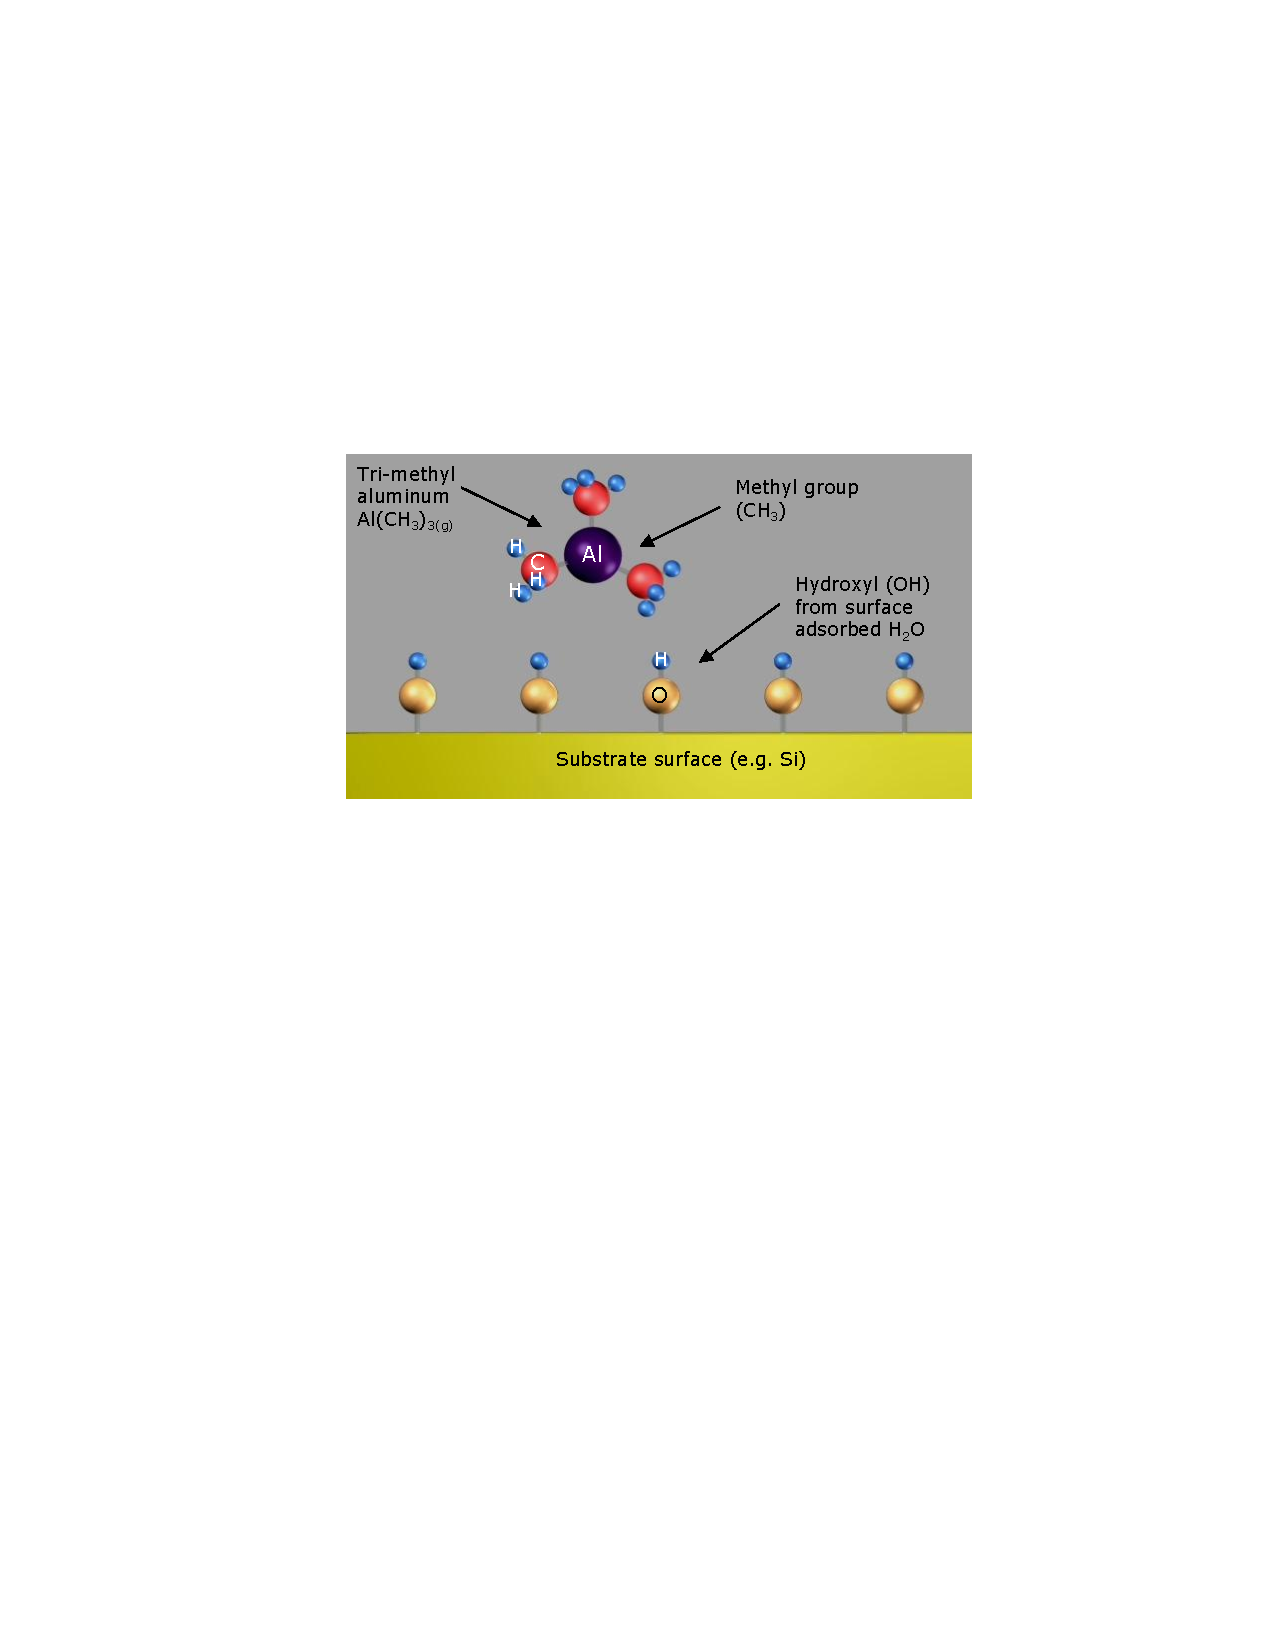
\includegraphics[width=0.45\linewidth]{./figures/synthesis/TMA1}%
	} 
	\hspace{6pt}
  \subfloat[][Precursor reaction]{%
%   	\label{fig:Q50-image}%
	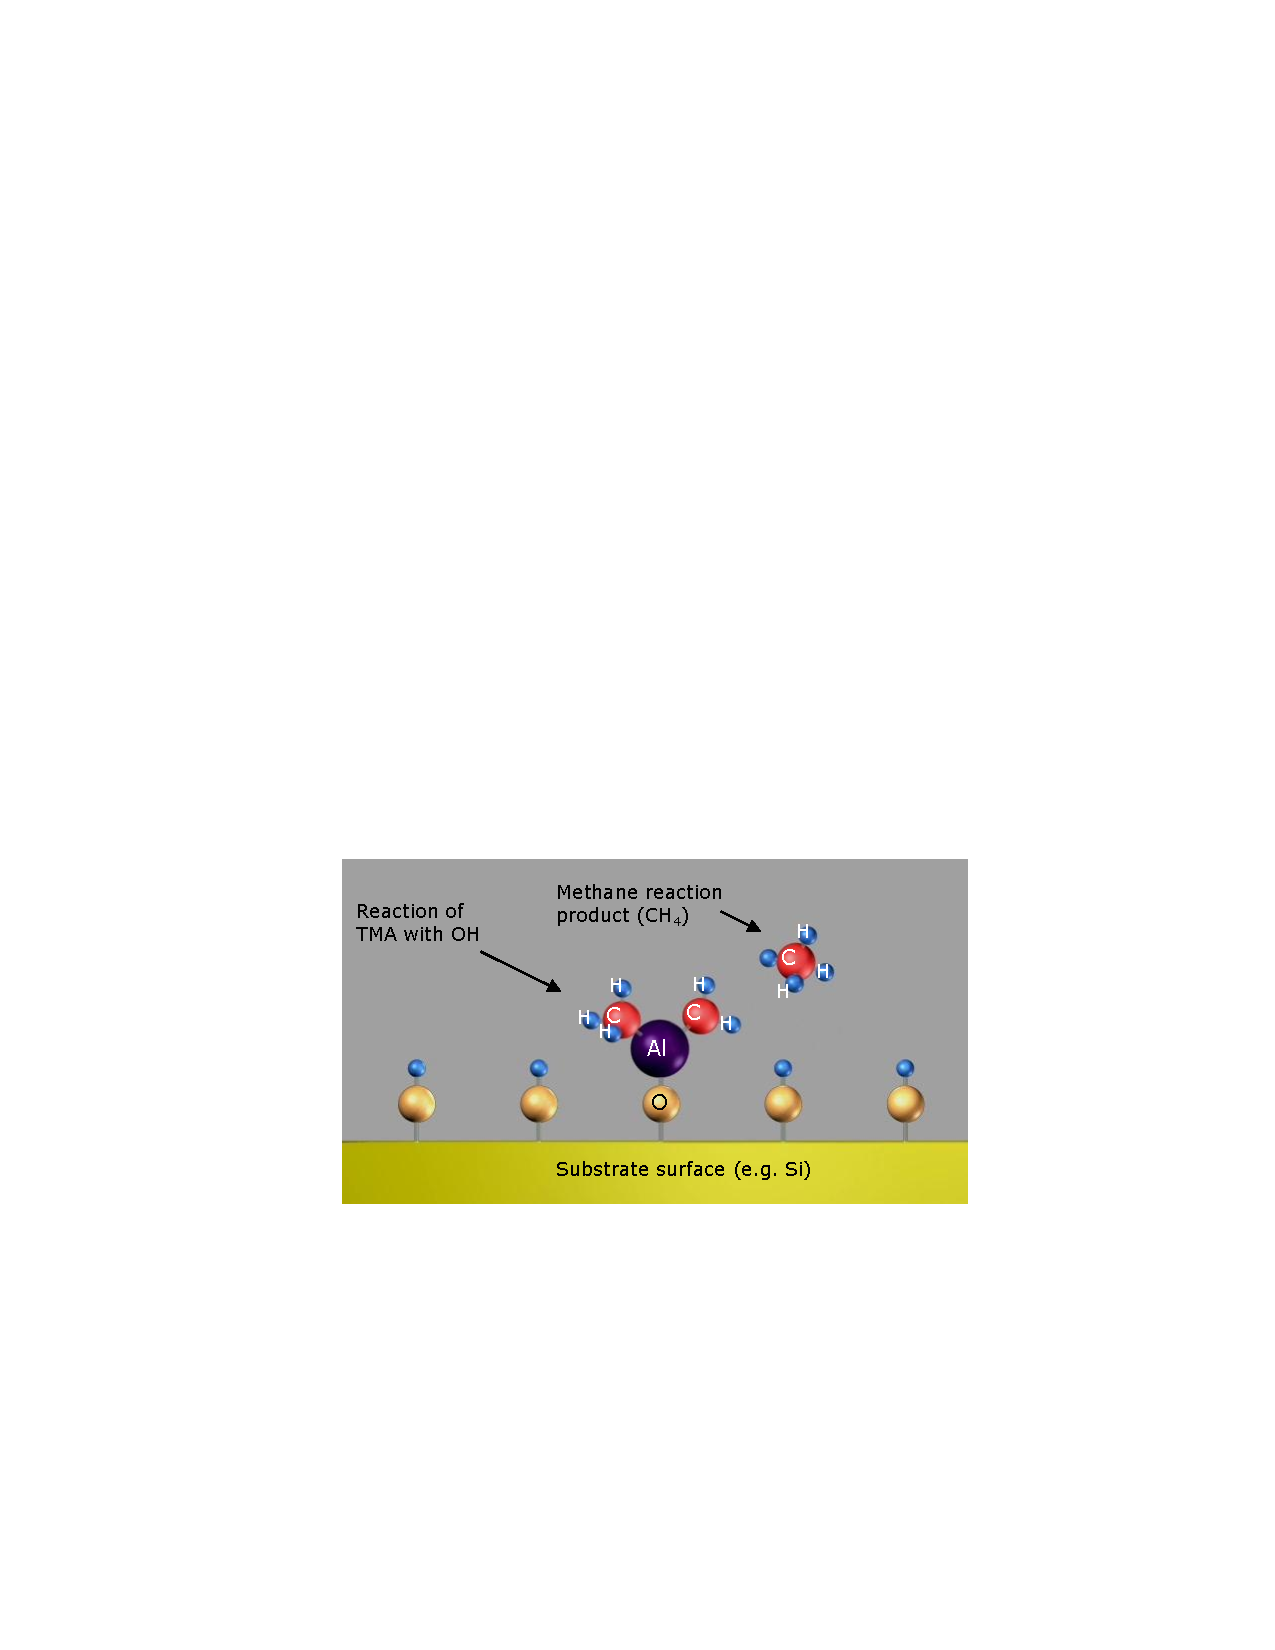
\includegraphics[width=0.45\linewidth]{./figures/synthesis/TMA2}%
	} \\
  \subfloat[][Reactor Purging]{%
%   	\label{fig:Q50-image}%
	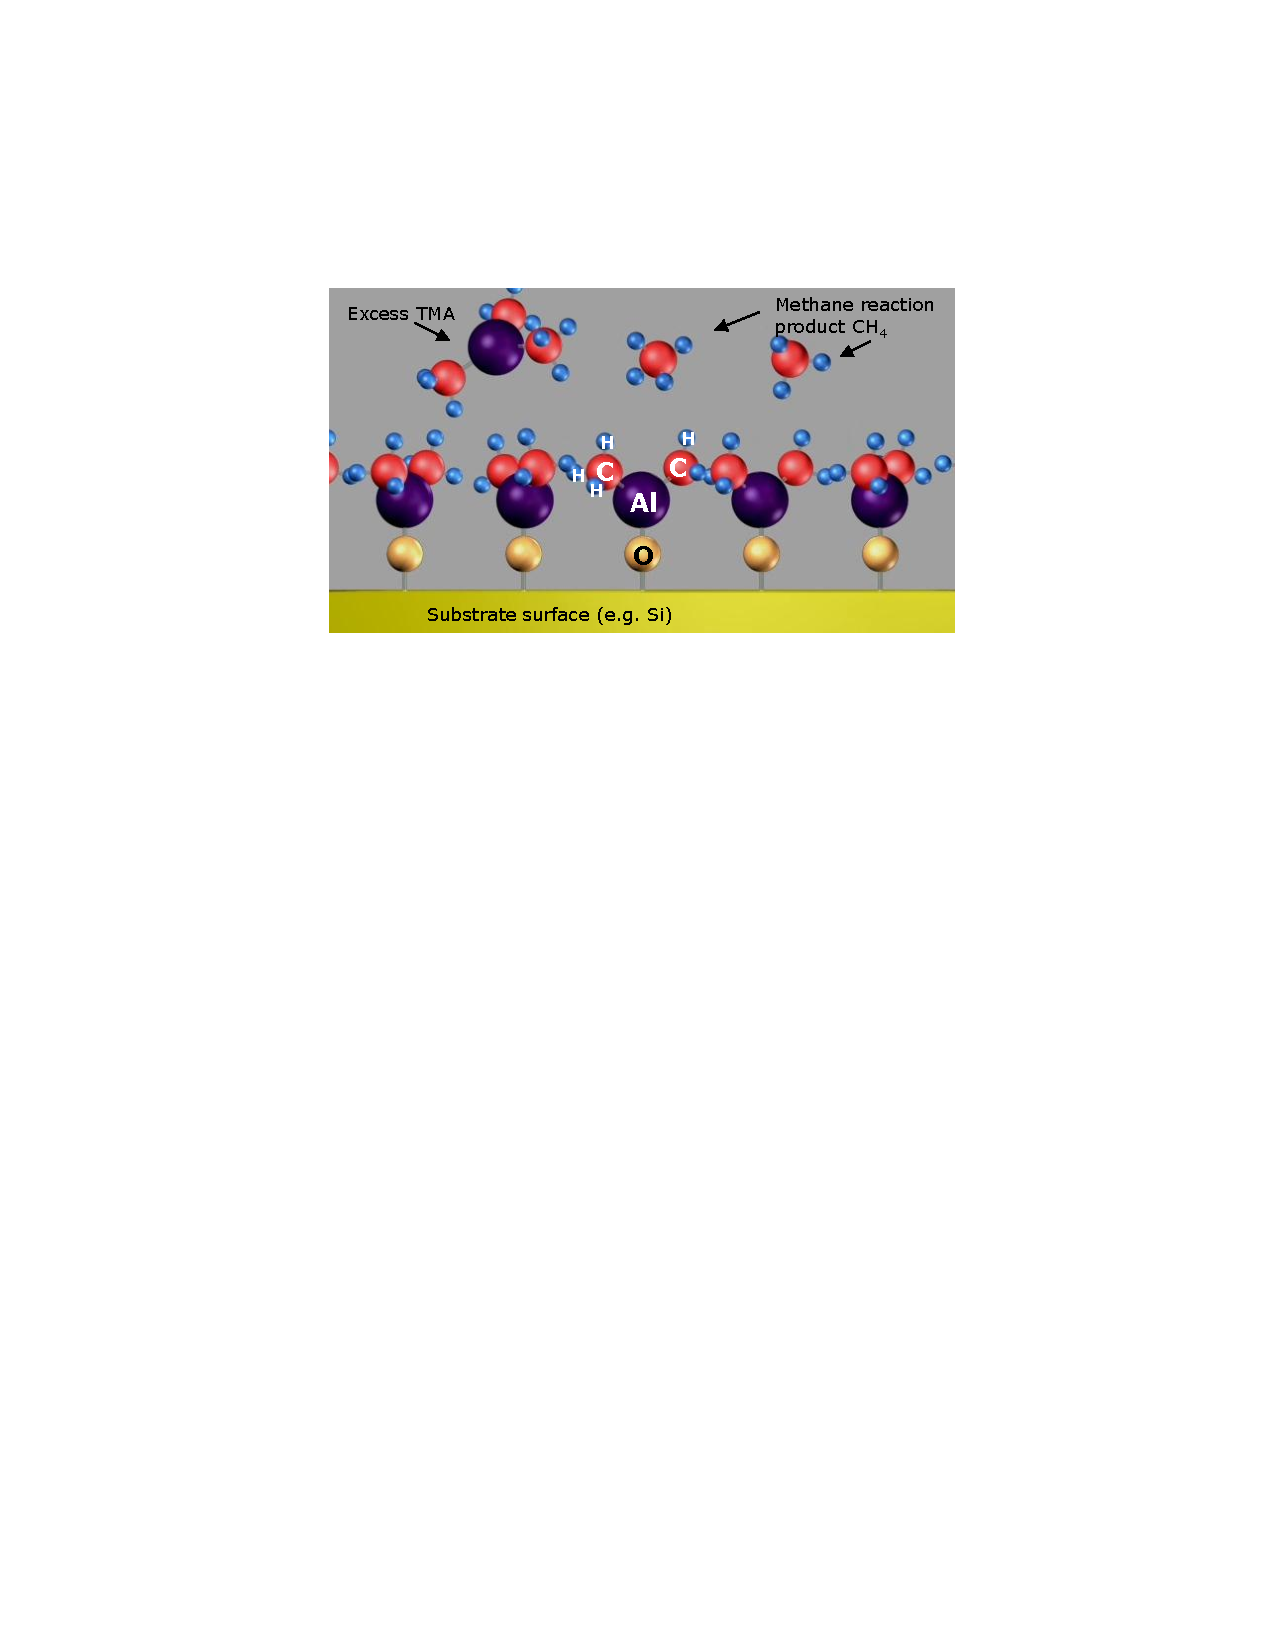
\includegraphics[width=0.45\linewidth]{./figures/synthesis/TMA3}%
	}  
	\hspace{6pt}	
  \subfloat[][Oxidant Injection]{%
%   	\label{fig:Q2000-image}%
	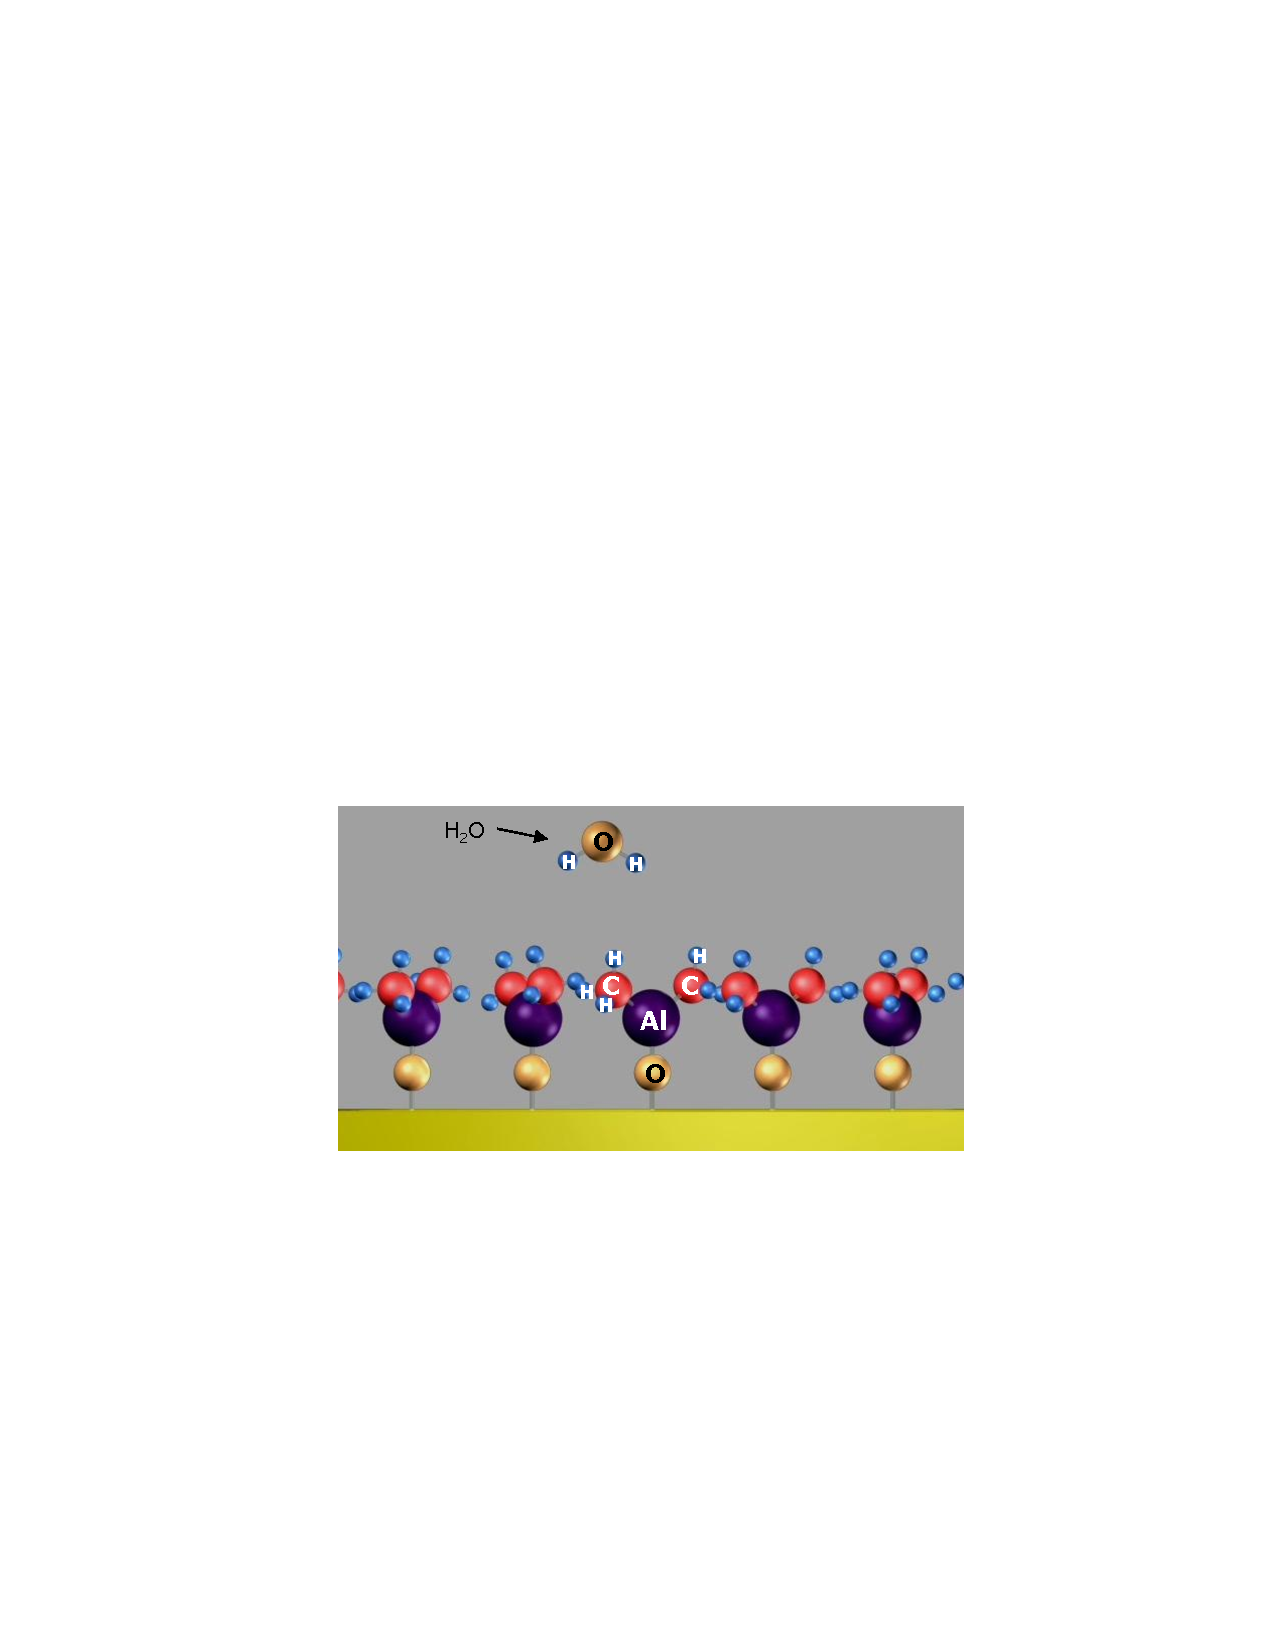
\includegraphics[width=0.45\linewidth]{./figures/synthesis/TMA4}%
	} \\
  \subfloat[][Oxidation Reaction (Ligand Exchange)]{%
%   	\label{fig:Q2000-image}%
	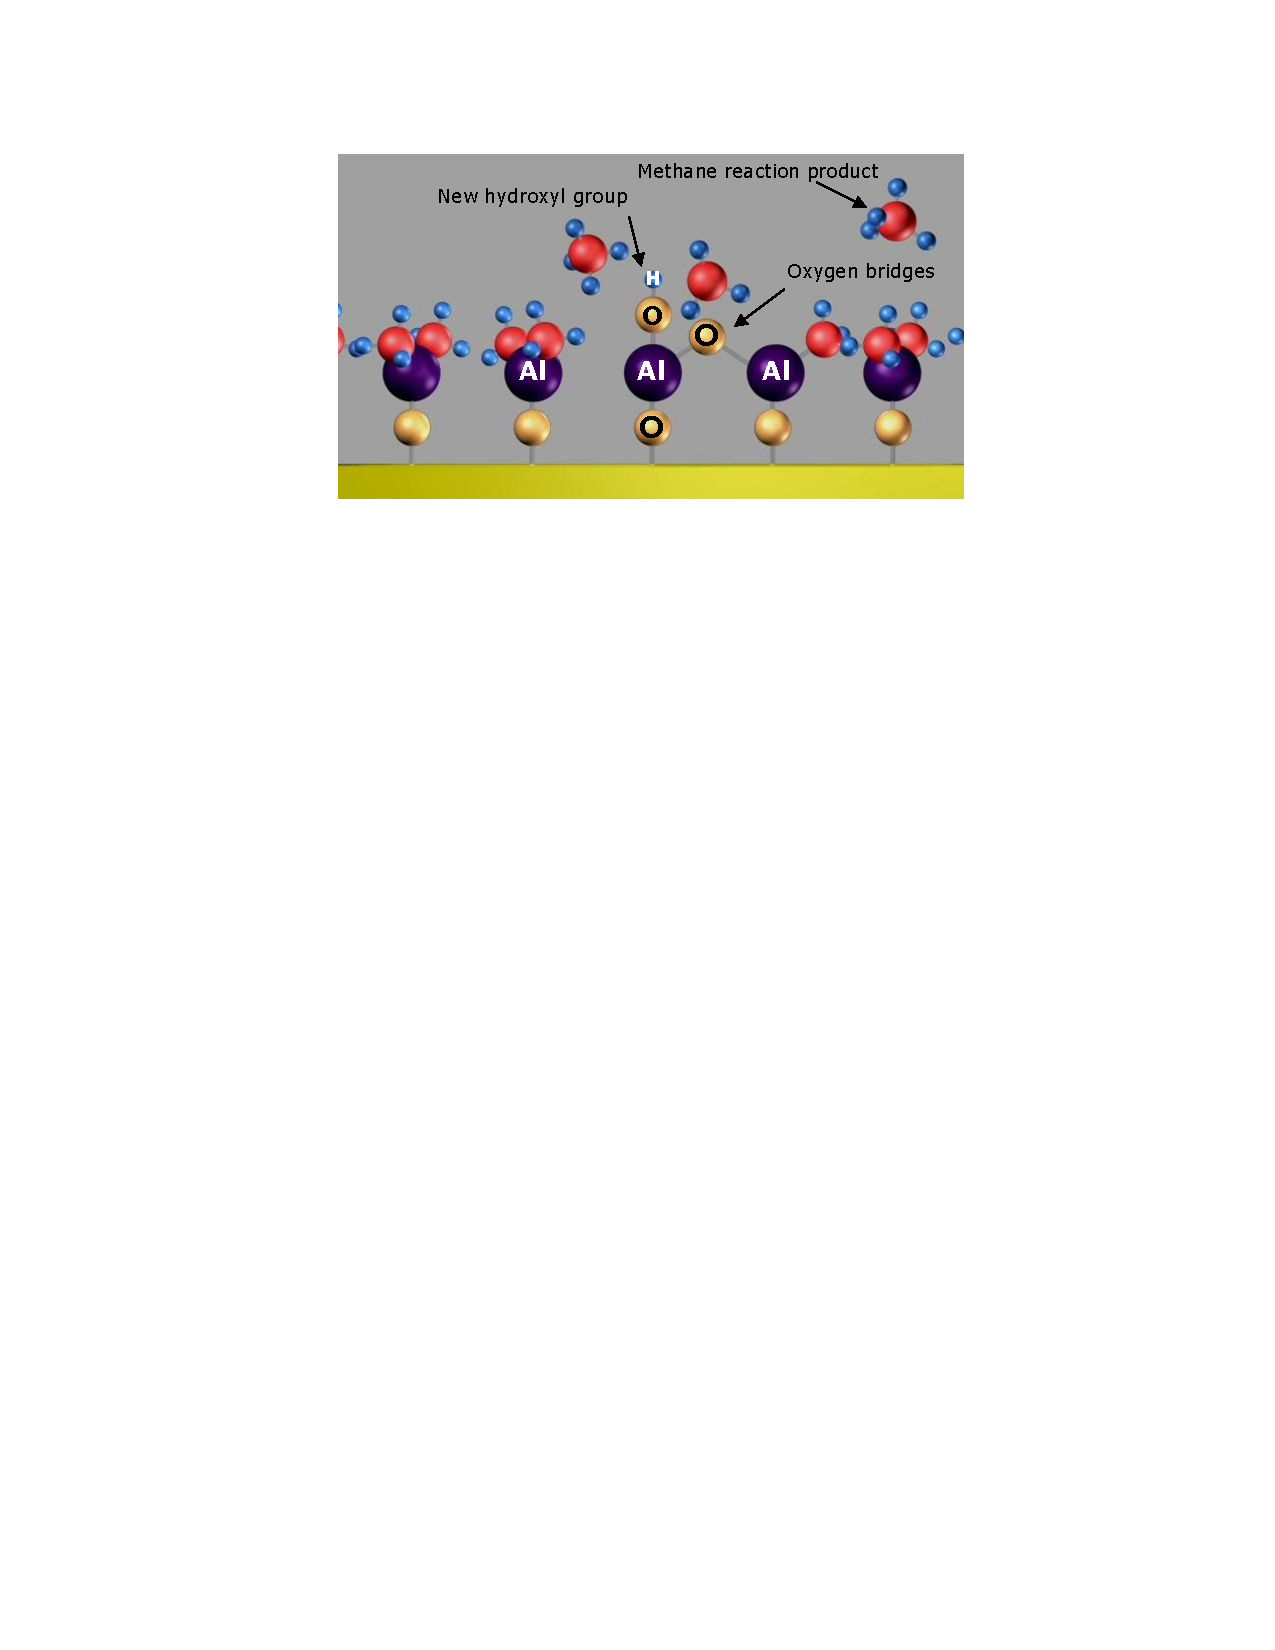
\includegraphics[width=0.45\linewidth]{./figures/synthesis/TMA5}%
	} 
	\hspace{6pt} 
  \subfloat[][Completed Cycle, Regenerated Surface]{%
%   	\label{fig:Q2000-image}%
	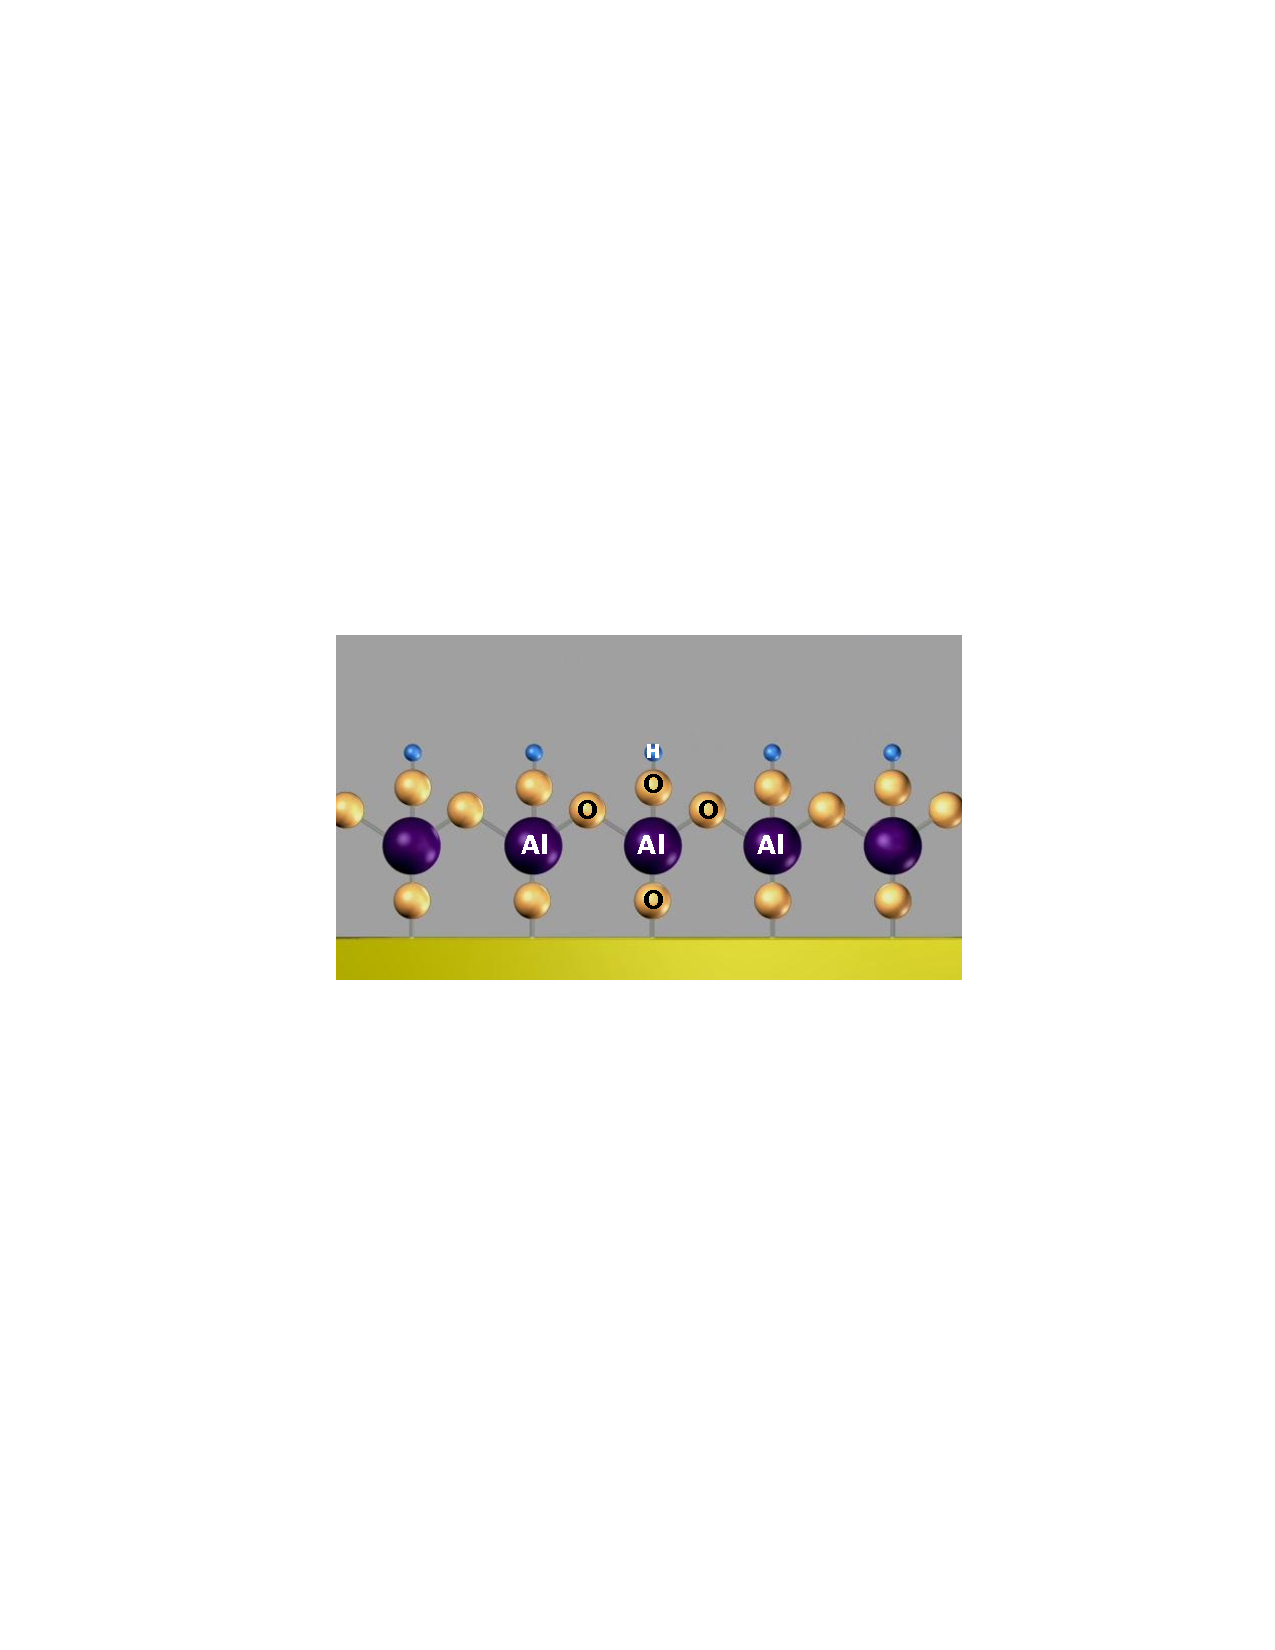
\includegraphics[width=0.45\linewidth]{./figures/synthesis/TMA6}%
	} 	
   \caption[Illustration of Example ALD Cycle]%
   		{Example schematic of the process of an ALD deposition cycle. This example\\%
		illustrates the reaction of TMA and water to form alumina (\ce{Al2O3}). \\%
		{\tiny Graphics reprinted with permission of Cambridge NanoTech, Inc.}\cite{CNT-web}}
   \label{fig:TMA-illustration}
\end{figure}

Having only surface reactions be permitted, as opposed to CVD where gas-phase interactions dominate, affords ALD a number of unique characteristics. One of these is the concept of the ``self-limiting'' growth mode.\cite{ALD-Handbook} This behavior arises from the limited number of available reaction sites; when all of these have either been reacted with or made unavailable by a blocking mechanism such as stearic hindrance from other local chemisorbed precursor the reaction can no longer proceed. At this point, additional available precursor is not going to be utilized, and instead will be removed and treated as waste material. The system is then evacuated, and a inert purge gas such as dry nitrogen or argon is flowed through the reactor. The purge gas serves both to push any remaining gases out of the reactor as well as to help desorb physisorbed species from the surface. The system would then again be evacuated, and the oxidant introduced and then pumped away to complete the cycle. Because of the self-limiting behavior of the reactants it is possible, in fact preferable, to utilize reactants that have highly energetic reactions with their corresponding surface site. For ALD, having fast and energetic reactions allows for rapid completion of the half-cycle, which allows for faster cycle times and thus higher throughputs. In CVD such energetic reactions are very difficult to control, and instead precursors that have only mild reactions --- with a Gibbs free energy exchange as close to zero as possible while remaining negative --- with each other are preferred. These require more effort to develop and require that the process be carefully controlled, as the reactions often can either easily extinguish themselves or rapidly accelerate in different conditions.\cite{ALD-Handbook}

In the implementation of most ALD systems, the purge gas is also used as a carrier gas for the precursors. Thus a constant flow of gas is passed through the system, instead of having it occasionally fully evacuated, and the precursor is able to be delivered from its source to the reactor more effectively. For some precursor compounds, in particular those with a low vapor pressure, having carrier-assisted transportation can greatly improve the behavior of the system.\cite{ALD-Handbook} 

Because of the self-limiting behavior, each deposition cycle is limited to a theoretical maximum of one monolayer of material (in practice a much lower coverage per cycle is attained), which is far less than a unit cell.\cite{ALD-Handbook} Generally per cycle growth rates range between 0.03--1.5 \AA{}, with the rate being nearly invariable during most of the deposition. This gives the second defining characteristic of ALD: very high (\AA\ level) thickness resolution. The downside of this aspect is that growths are generally much slower than other types of depositions; ALD is generally slower by an order of magnitude or more than a similar CVD process, as an example. This has proved invaluable in many processes where high precision is critical, such as electronics manufacturing. Intel, for example, uses ALD to deposit extremely precise layer thicknesses of a high-$\kappa$ dielectric (such as hafnia, \ce{HfO2}) for use as the gate oxide in transistors.\cite{toriumi_application_2008,chen_atomic_2007}

There are a wide range of binary oxides for which ALD processes have been developed. A deposition for alumina (\ce{Al2O3}, one of the first ALD materials developed, was discussed briefly above and the method is is common use.\cite{lee_al2o3_2003,puurunen_surface_2005} High-$k$ gate oxides such as hafnia and zirconia (\ce{ZrO2}), along with some of their nitrides and silicides, are under intense research to develop industrial processes for their use in integrated circuitry.\cite{toriumi_application_2008,chen_atomic_2007} Other transition metal oxides, such as titania (\ce{TiO2}) and iron oxide (\ce{Fe2O3}), have also had ALD deposition processes developed for their deposition. \cite{lim_atomic_2003,scheffe_atomic_2009}

The methods described above will produce a layer of a binary oxide material (\ce{AO_{x}}); if more complex materials are desired the method must be changed. The basic principles remain the same; one would perform the procedure for depositing a cycle of a binary oxide and then change the precursor and deposit another cycle of a different oxide material. For example, if one wished to deposit \PTO{}, one would begin by depositing a layer of \ce{TiO2} and then depositing a layer of lead oxide (\ce{PbO}). Repeating this set of cycles --- a super-cycle --- would eventually form an ternary oxide film. 

However, deposition of \ce{ABO3} oxides is not this simple in practice. In many cases, running each oxide cycle in a 1:1 ratio will deposit a non-stoichiometric material. This makes it necessary to modify the method to deposit more of one type of oxide than the other. For example, if a material is Ti-rich the super-cycle ratio would be modified to increase the number of lead oxide cycles as compared to the titania cycles. Careful tuning of the deposition conditions, which include a variety of different factors, is required to obtain a desired and consistent film stoichiometry. 

In addition to lead titanate, there are other ternary oxide systems that are being investigated. Examples of which are bismuth ferrite (\ce{BiFeO3}) or barium strontium titanate (\ce{(Ba\,Sr)TiO3}).\cite{chu_nanoscale_2009}

ALD reactions are rather sensitive to a number of factors, such as temperature. The temperature must be high enough that the reactants have sufficient energy to drive the surface reaction but not so high as to allow undesirable reactions to activate (e.g. precursor cracking or surface material desorption). Precursor selection is also very important, for similar reasons. The precursors must also be incapable of reacting with themselves, to allow the self-limiting mechanism to work properly.\cite{ALD-Handbook}


%
%\begin{subreactions}
%	\label{chem:2TMA}
%	\begin{reactions}
%		Al(CH3)3 + M-OH_{surf} &-> M-O-Al(CH3)2_{\,surf} + CH4 \label{chem:2TMA1} \\
%		M-O-Al(CH3)2_{\,surf} + 2H2O &-> M-O-Al(OH)2_{\,surf} + 2CH4 \label{chem:2TMA2}
%	\end{reactions}
%\end{subreactions}
%
%\begin{subreactions}
%\newcommand*{\thesubequation}{(\reactiontag.\alph{equation})}
%\label{chem:TMA}
%\begin{align}
%	\cee{Al(CH3)3 + M-OH_{surface} &-> M-O-Al(CH3)2_{\ surf} + CH4}%
%		\label{chem:TMA1}
%		\\
%	\cee{M-O-Al(CH3)2_{\ surf} + 2H2O &-> M-O-Al(OH)2_{\ surf} + 2CH4}%
%		\label{chem:TMA2}
%\end{align}
%\end{subreactions}



\lipsum







